\documentclass{article}
\usepackage[utf8]{inputenc}
\usepackage[left=3cm, right=3cm, top=3cm]{geometry}
\usepackage{graphicx}
\begin{document}

    \begin{titlepage}
      \centering
        \vfill
        {\bfseries\Huge
          PROJECT 4: BAGELS \\
            \vskip2cm
          }

          {\bfseries\Large
            IN THIS PROJECT, YOU WILL USE AN LCD SCREEN TO PLAY A CLASSIC
            MATHEMATICAL LOGIC GAME, BAGELS\\
          } {
            \vskip1cm
        }
        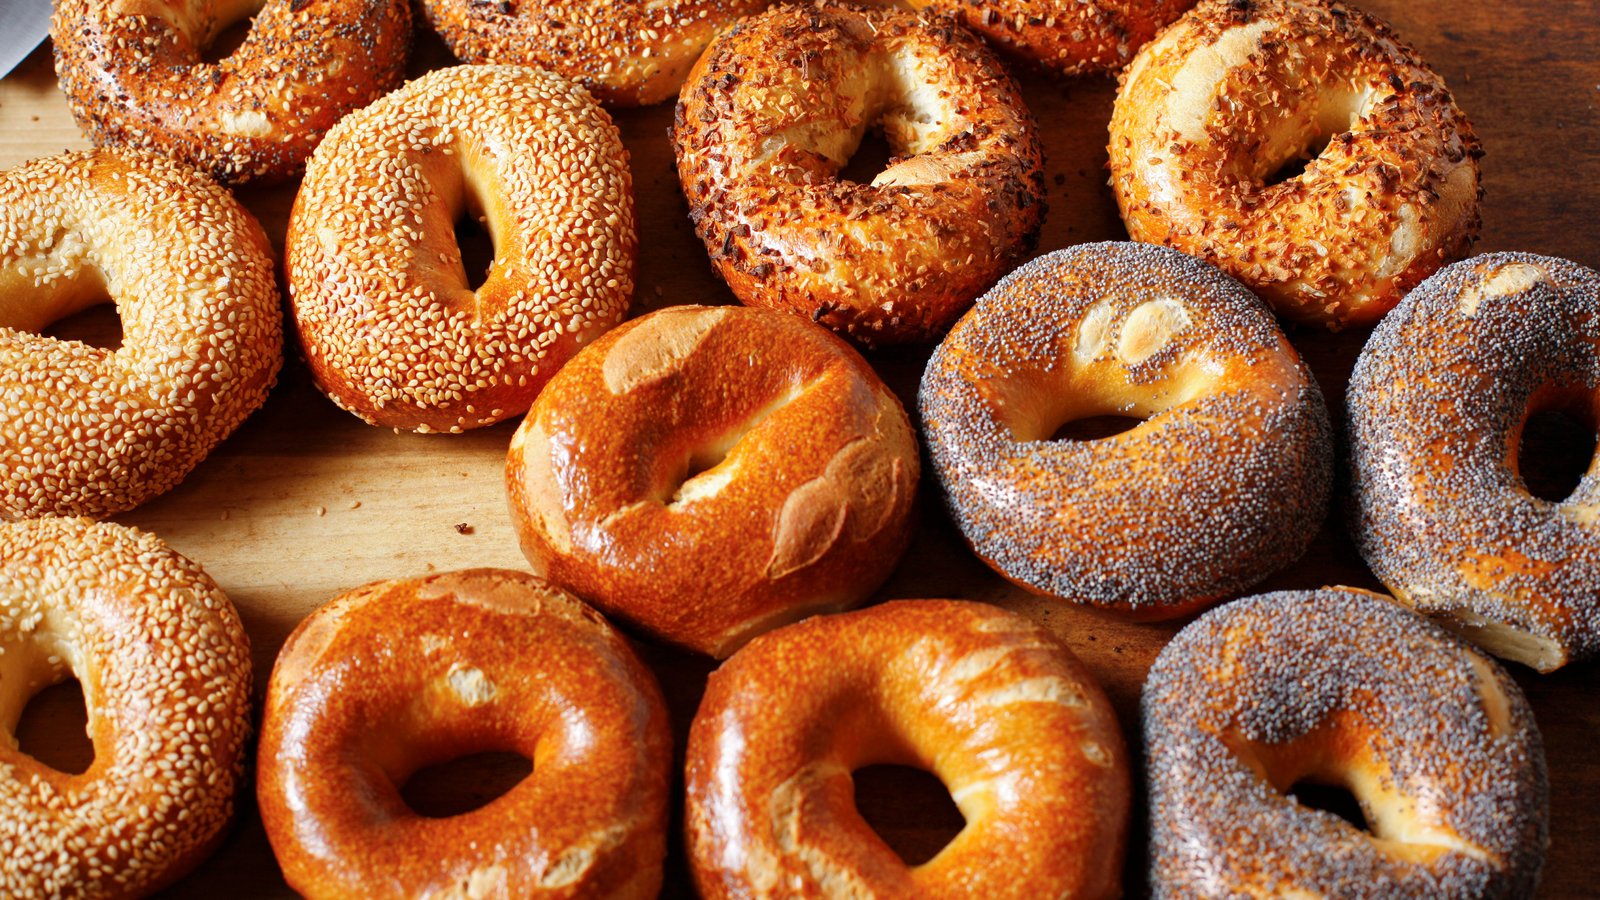
\includegraphics[width=\textwidth]{bagels.jpg}
        \vfill
        \vfill
    \end{titlepage}
\newpage

\section{Objectives}\label{sec:objectives}
At the end of this activity, students will be able to:

\begin{itemize}
\item {Perform mathematical deduction in simple contexts.}
\item {Regain a sense a childlike wonder about math and BAGELS in general.}
\end{itemize}

\section{Parts Required}\label{sec:parts}

\begin{itemize}
\begin{minipage}{0.4\linewidth}
\item Arduino board
\item Breadboard
\item LCD screen
\item Potentiometer
\end{minipage}
\end{itemize}

\section{Setup}
\begin{enumerate}
\item {Download, unzip, and install the Arduino Integrated Development Environment
    (IDE) from https://www.arduino.cc/en/Main/Donate (does not need admin
    privileges).}
\item {Gather all the necessary parts listed in Sec. \ref{sec:parts}}.
\end{enumerate}

\section{How it Works}
BAGELS is a number guessing game. For each guess, you will be told:

\begin{enumerate}
\item {\textbf{Fermi} correct digit placed correctly.}
\item {\textbf{Pico} correct digit placed incorrectly.}
\item {\textbf{BAGELS} no digits are correct.}
\end{enumerate}

The goal is to guess the number in the fewest average number of tries (i.e. you play
10 games, add up how many guesses it took for each one, and then divide by 10 to get
your average).

\vspace{1cm}

Here is an example game, if the secret \# is 029:

\vspace{1cm}

\begin{tabular}{c| c| c}
  \hline
  Guess &	Result &	comment \\
  \hline
  376	& BAGELS &	No digits correct\\
  914	& Pico	&1 digit correct but in wrong place\\
  820	& Fermi &Pico	2 digits correct, but 1 in wrong place\\
  \dots	& (keep guessing) &\\
  092	& Fermi Pico Pico &	All digits correct, 2 in wrong places\\
  029	& Fermi Fermi Fermi & You won!!!\\
\end{tabular}

\newpage

\section{Building the Circuits}
The schematic for the circuits you will be building is below. The keypad is
approximated as a gray-green blob because that specific part did not exist in the
schematic drawing library :-(.

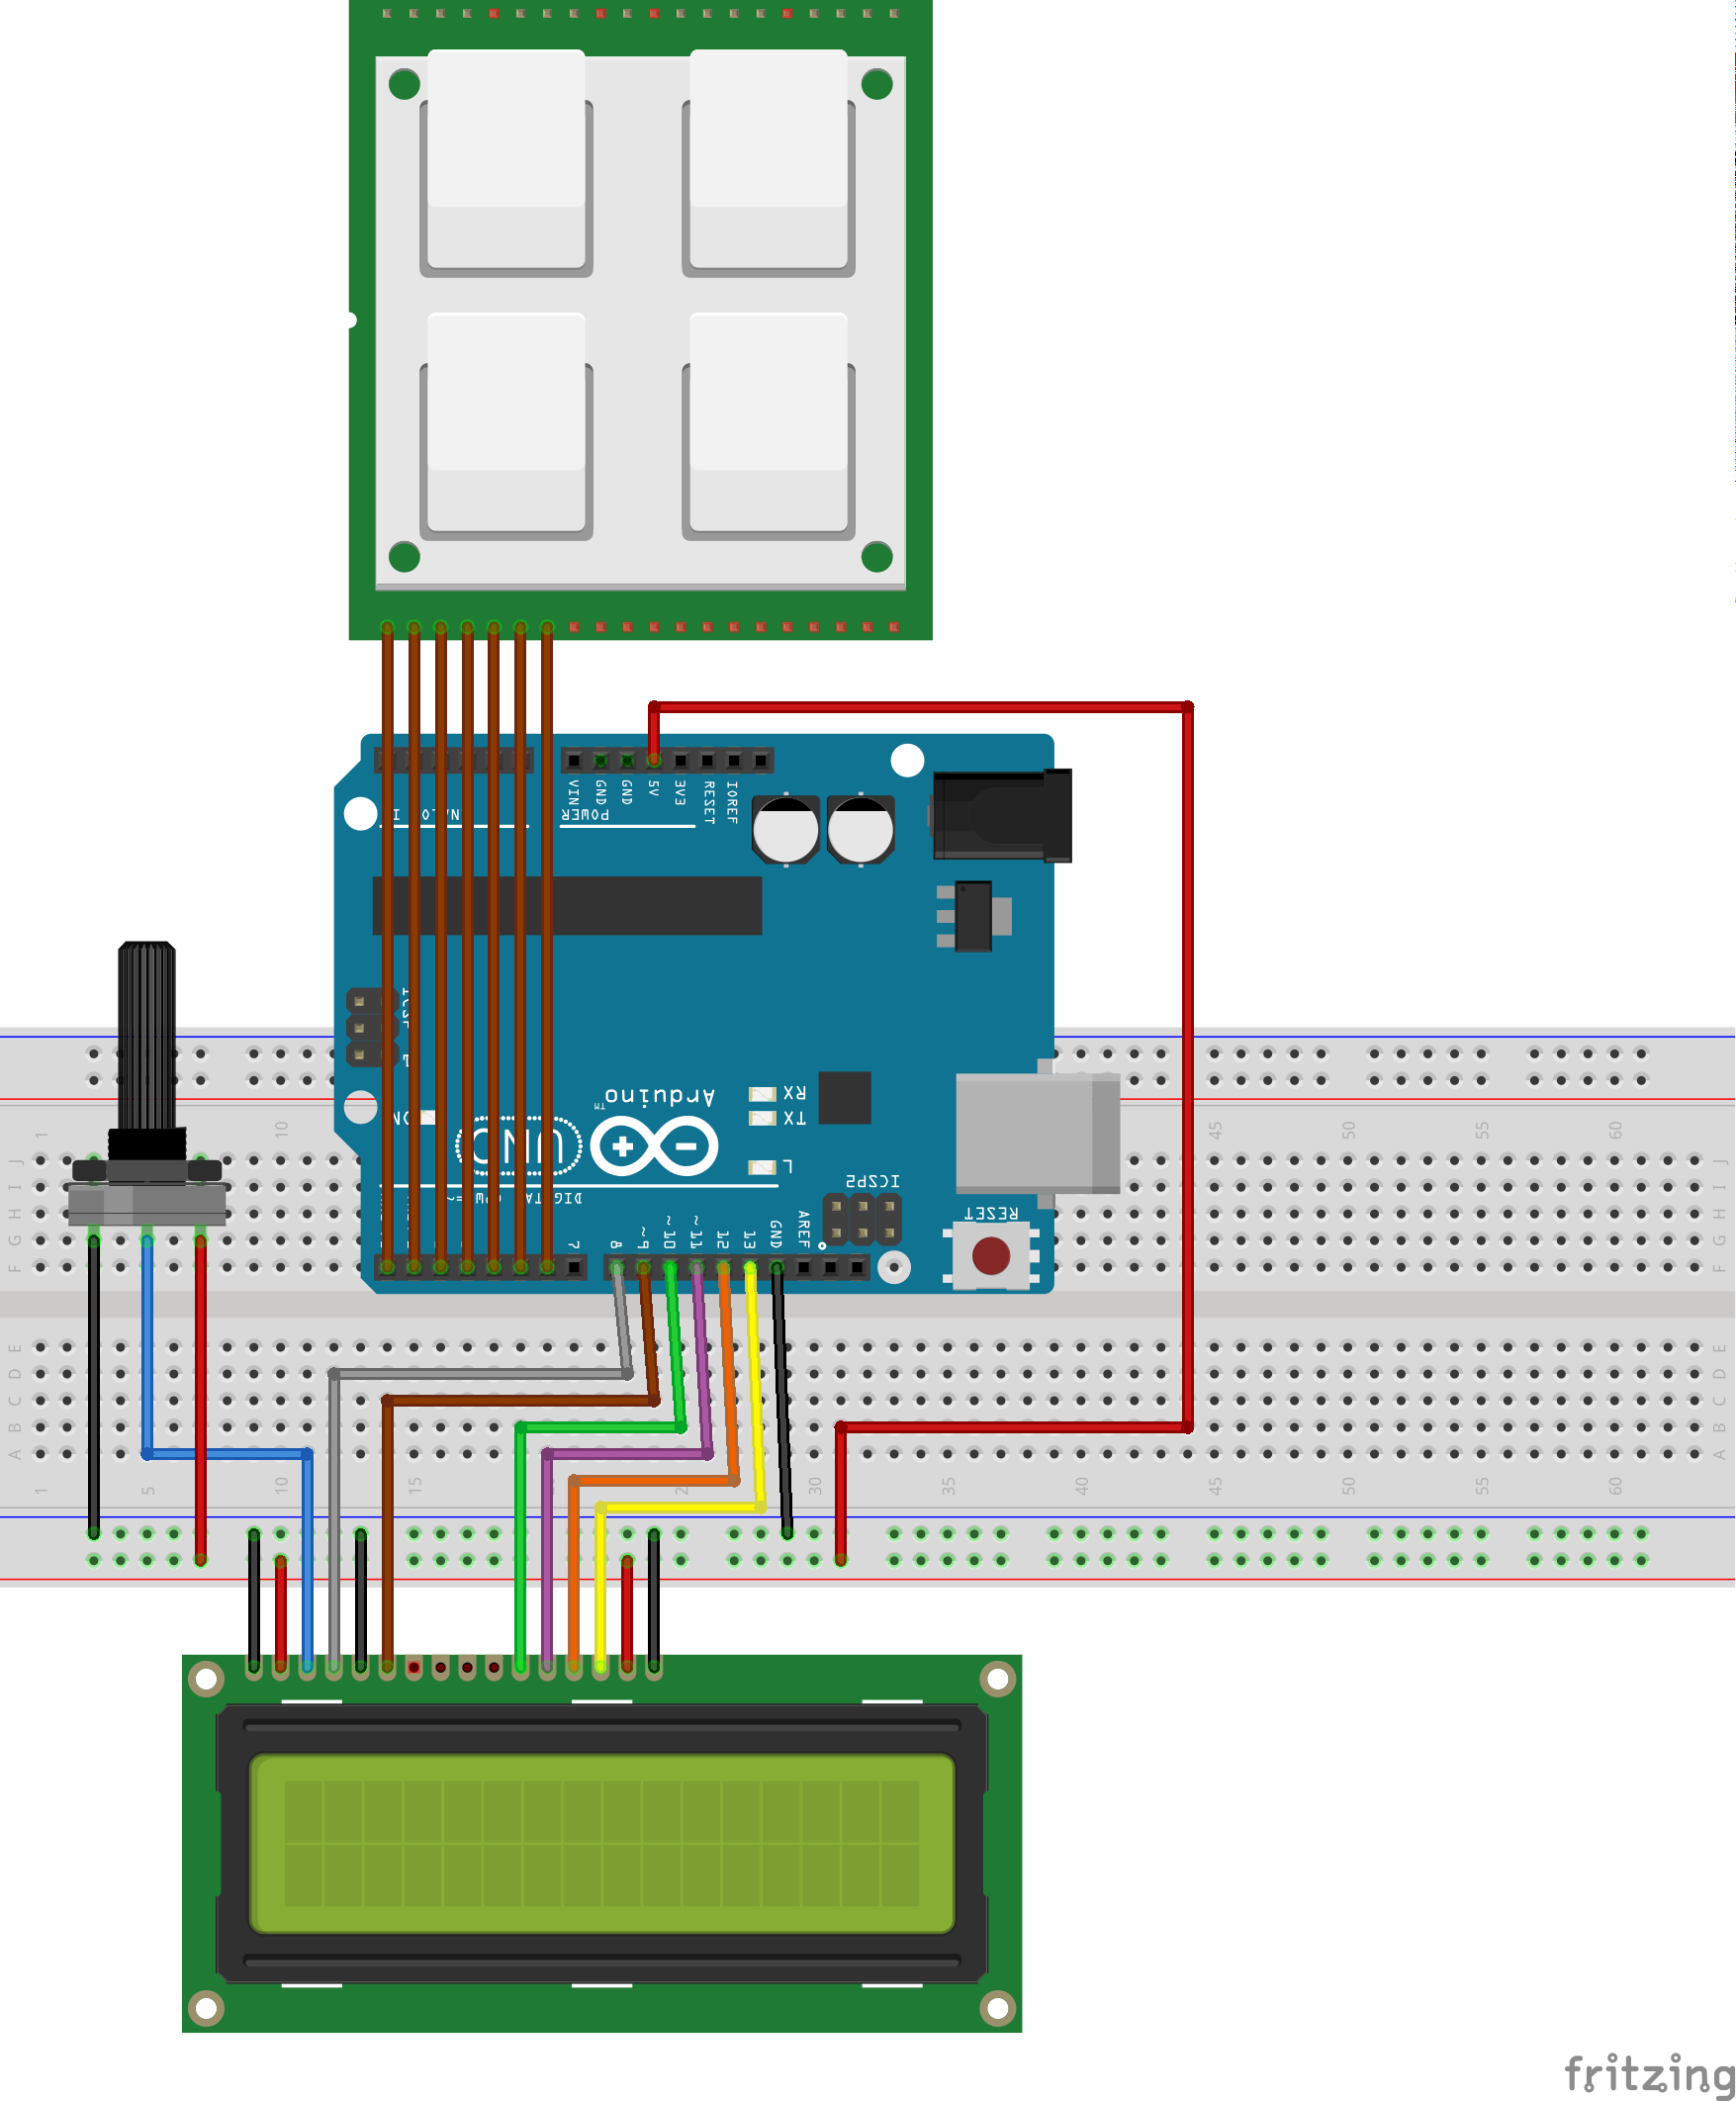
\includegraphics[width=\textwidth]{exp6-bagels_bb.png}

\section{Programming the Arduino}
The base code for programming the Arduino is provided. Using the Arduino IDE, open
the .ino file.  The IDE allows you to do 4 things: edit the code, verify the code
(i.e. does not contain syntax errors), upload the code to the Arduino, and view the
diagnostic output. To upload to the Arduino, just click the upload button!

\section{Extending the Code}

Once you gotten the hang of the game, try changing it to only generate 2 (or 4!)
digit numbers. How many lines of code did you have to change?

\end{document}
